\documentclass[serif]{beamer}

\usepackage{xeCJK}

\usepackage{amsfonts} %额外的数学符号,花体,俄文德文字母

\usepackage{amssymb}

\newcommand\hmmax{0} % default 3

% \newcommand\bmmax{0} % default 4

\usepackage{bm}

\usepackage{amsthm,amsmath,amssymb}

\usepackage{mathrsfs}

\usepackage{latexsym}

\usepackage{geometry}

\usepackage{fancyhdr}

\usepackage{mathtools}

\usefonttheme{professionalfonts}%把所有的字体间距变正常,和article一样

\usetheme{Berlin}

\usecolortheme{whale}

\useinnertheme[shadow=true]{rounded}

\usefonttheme[onlymath]{serif}% 默认的数学公式较难看,使用serif可以使得公式的样式变为常用latex的公式样式

% 1.1内部主题在这里,内部主题主要控制的是标题页,列表项目、定理环境、图表环境、脚注在一帧内的内容格式(做幻灯片的时候,其实一般不建议使用脚注)。预定义的内部主题格式有default、circles、rectangles、rounded、inmargin等。

%1.2外部主题 外部主题主要控制的是幻灯片顶部尾部的信息栏、边栏、图标、帧标题等一帧之外的格式。预定义的外部主题有default、infolines、miniframes、smoothbars、sidebar、split、shadow、tree、smoothtree等。

%1.3色彩主题 色彩主题控制各个部分的色彩。预定义的色彩主题包括default、albatross、beaver、beetle、crane、dolphine、dove、fly、lily、orchid、rose、seagull、seahorse、sidebartab、structure、whale、wolverine等。

\setbeamercovered{transparent}

% 也可删去

\setbeamertemplate{navigation symbols}{} % 取消导航图标

\setbeamertemplate{footline}{%

\leavevmode%

\hbox{%

\begin{beamercolorbox}[wd=.233333\paperwidth,ht=2.25ex,dp=1ex,center]{author in head/foot}%

\usebeamerfont{author in head/foot}\insertshortauthor

\end{beamercolorbox}%

\begin{beamercolorbox}[wd=.533333\paperwidth,ht=2.25ex,dp=1ex,center]{title in head/foot}%

\usebeamerfont{title in head/foot}\insertshorttitle

\end{beamercolorbox}%

\begin{beamercolorbox}[wd=.233333\paperwidth,ht=2.25ex,dp=1ex,right]{date in head/foot}%

\usebeamerfont{date in head/foot}\insertshortdate{}\hspace*{2em}

\insertframenumber{} / \inserttotalframenumber\hspace*{2ex}

\end{beamercolorbox}}%

\vskip0pt%

}% 重设下方导航条并增加页码

\newcommand{\song}{\CJKfamily{song}} % 宋体 (Windows自带simsun.ttf)

\newcommand{\fs}{\CJKfamily{fs}} % 仿宋体 (Windows自带simfs.ttf)

\newcommand{\kai}{\CJKfamily{kai}} % 楷体 (Windows自带simkai.ttf)

\newcommand{\hei}{\CJKfamily{hei}} % 黑体 (Windows自带simhei.ttf)

\newcommand{\li}{\CJKfamily{li}} % 隶书 (Windows自带simli.ttf)

\newcommand{\you}{\CJKfamily{you}} % 幼圆 (Windows自带simyou.ttf)

\newcommand{\chuhao}{\fontsize{42pt}{\baselineskip}\selectfont} % 字号设置

\newcommand{\xiaochuhao}{\fontsize{36pt}{\baselineskip}\selectfont} % 字号设置

\newcommand{\yichu}{\fontsize{32pt}{\baselineskip}\selectfont} % 字号设置

\newcommand{\yihao}{\fontsize{28pt}{\baselineskip}\selectfont} % 字号设置

\newcommand{\erhao}{\fontsize{21pt}{\baselineskip}\selectfont} % 字号设置

\newcommand{\xiaoerhao}{\fontsize{18pt}{\baselineskip}\selectfont} % 字号设置

\newcommand{\sanhao}{\fontsize{15.75pt}{\baselineskip}\selectfont} % 字号设置

\newcommand{\sihao}{\fontsize{14pt}{\baselineskip}\selectfont} % 字号设置

\newcommand{\xiaosihao}{\fontsize{12pt}{\baselineskip}\selectfont} % 字号设置

\newcommand{\wuhao}{\fontsize{10.5pt}{\baselineskip}\selectfont} % 字号设置

\newcommand{\xiaowuhao}{\fontsize{9pt}{\baselineskip}\selectfont} % 字号设置

\newcommand{\liuhao}{\fontsize{7.875pt}{\baselineskip}\selectfont} % 字号设置

\newcommand{\qihao}{\fontsize{5.25pt}{\baselineskip}\selectfont} % 字号设置



\begin{document}

\title[title]{GenCNN: Neural Network with 100\% Accuracy for Cycle Recognization Task}

\author[]{Jiaming Shan} % 显示作者

\institute[Sch]{

	Shanghai Jiao Tong University }

\date[Date below]{Shanghai, 2022} % 显示日期

%%%%%%%%%%%%%%%%%%%%%%%%%%%%%%%%%%%%%%%%%%%%%%%%%%%%%%%%%%%%%%%%

\begin{frame}

	\thispagestyle{empty}%去掉封面的页眉页脚

	\titlepage

\end{frame}

%%%%%%%%%%%%%%%%%%%%%%%%%%%%%%%%%%%%%%%%%%%%%%%%%%%%%%%%%%%%%%%%

\begin{frame}{Content}

	\tableofcontents % 显示目录,并超链接到对应的section

\end{frame}

%%%%%%%%%%%%%%%%%%%%%%%%%%%%%%%%%%%%%%%%%%%%%%%%%%%%%%%%%%%%%%%%

\section{Problem}

\begin{frame}{Problem}

	If we generate a dataset which is easy for human to achieve 100\% accuracy, can we get a model with 100\% accuracy?

	Probalbly not.

\end{frame}

\begin{frame}{Cycle Dataset}

	\begin{itemize}

		\item We build a cycle dataset.

		\item 60000 train images, 10000 test images.

		\item Each image has size 28x28, with every pixel 0 or 1.

		\item The label of a image is 0 or 1,
		      0 means there is no cycle, 1 means there is a cycle.

	\end{itemize}

\end{frame}

\begin{frame}{}

	Here are some samples:

	\begin{figure}[H] %H为当前位置,!htb为忽略美学标准,htbp为浮动图形
		\centering %图片居中
		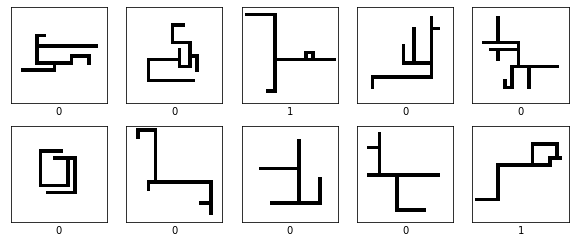
\includegraphics[width=1.0\textwidth]{../image/img10.png} %插入图片,[]中设置图片大小,{}中是图片文件名
		\caption{Cycle Dataset} %最终文档中希望显示的图片标题
		\label{Fig.Flow} %用于文内引用的标签
	\end{figure}

\end{frame}

\begin{frame}

	\begin{itemize}

		\item There exists deterministic algorithm to detect cycle.

		\item Can we build a deterministic neural network to detect cycle?

	\end{itemize}

\end{frame}

\section{Model Architecture}

\begin{frame}{BFS Algorithm}

	We can use BFS in "1" pixel to solve this problem!

	\begin{block}{Algorithm 1}

		BFS. If go to a visited node, then there is a cycle.

	\end{block}

	Problem: This algorithm may return in every step. Difficult to implement in a neural network.

	\begin{block}{Algorithm 2}

		BFS to get the distance of every node to the starting point.

		We can detect cycle easily by the distance image.

	\end{block}

	Easy to implement in neural network!

	We will implement Algorithm 2.


\end{frame}

\begin{frame}{Implement BFS Algorithm}

	\textbf{Initializer}:

	Choose a random "1" pixel and set its distance to $0$, and set all other pixels to $+\infty$.

	\textbf{Solver}:

	Input the distance data output by the initializer,

	and do distance propagation operation repeatedly until all distance remains unchanged.

	\textbf{Extractor}:

	Detect whether there are patterns a pixel with distance $d$ has at least two neighbor pixels with distance $d-1$.

	If there are, output $1$, showing that the image contains cycle, else output $0$.

\end{frame}

\begin{frame}

	\begin{figure}[H] %H为当前位置,!htb为忽略美学标准,htbp为浮动图形
		\centering %图片居中
		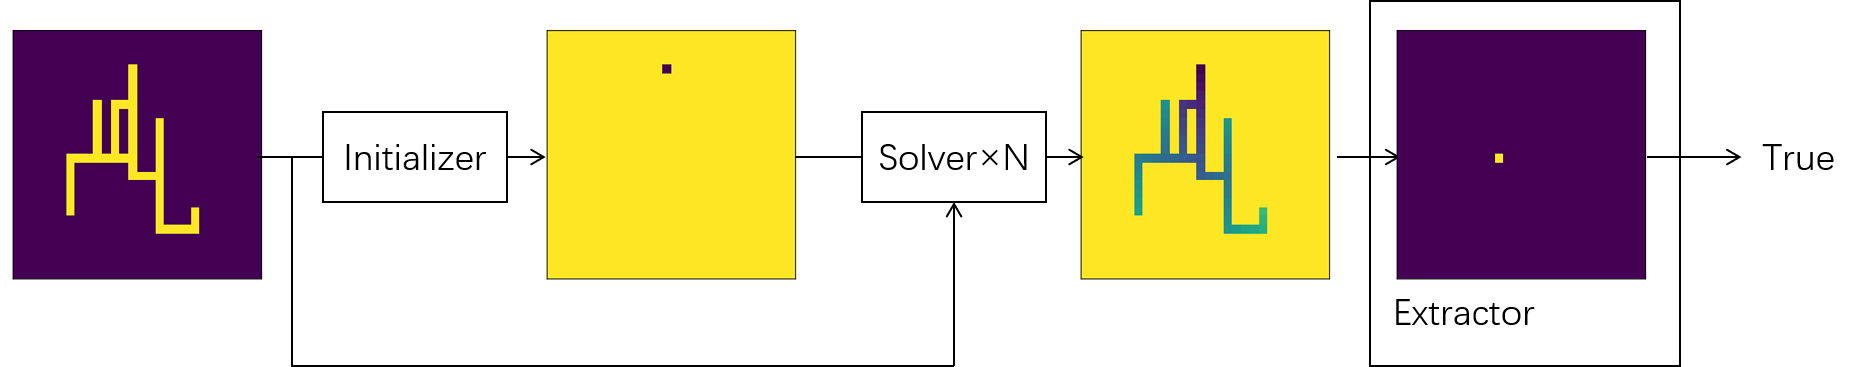
\includegraphics[width=1.0\textwidth]{../image/flow.png} %插入图片,[]中设置图片大小,{}中是图片文件名
		\caption{Data Flow of Deterministic Algorithm in Cycle Recognization} %最终文档中希望显示的图片标题
		\label{Fig.Flow} %用于文内引用的标签
	\end{figure}

\end{frame}

\begin{frame}{Solver Architecture}

	$d_{merge} = padding(d + inputs \cdot \infty, 1, 1, +\infty)$
	\begin{align*}
		d_{new}[i,j] = \min( & d_{merge}[i,j],        \\
		                     & d_{merge}[i+1, j] + 1, \\
		                     & d_{merge}[i-1, j] + 1, \\
		                     & d_{merge}[i, j+1] + 1, \\
		                     & d_{merge}[i, j-1] + 1)
	\end{align*}

	Notice that we use the same raw inputs in each solver.

	Call it global inputs.

\end{frame}

\begin{frame}{Extractor Architecture}

	\begin{align*}
		 & v = d[i,j]                                       \\
		 & l = [d[i,j-1], d[i-1,j], d[i+1,j], d[i,j+1]] - v \\
		 & d[i,j] = sum(l == -1) >= 2
	\end{align*}

    \begin{center}

    If any $d[i,j]$ outputs $1$, then there is a cycle, 
    
    and Extracor return $1$, else return $0$.

    \end{center}

\end{frame}


\begin{frame}{Turn BFS Algorithm to Neural Network}

	Solver and Extractor work like ConvNet!

	Call it GenConv.

	ConvNet: $x_{new} = \sigma(\Sigma w_ix_i + b)$. $x_i$ is a neighborhood point of $x$.

	GenConv: $x_{new} = f(X)$.

	We call $f$ GenKernel.

	It is a more generalized CNN.

	We call it GenCNN.

\end{frame}

\begin{frame}{Build GenCNN}

	\begin{figure}[H]
		\centering
		\begin{minipage}{.5\textwidth}
			\centering
			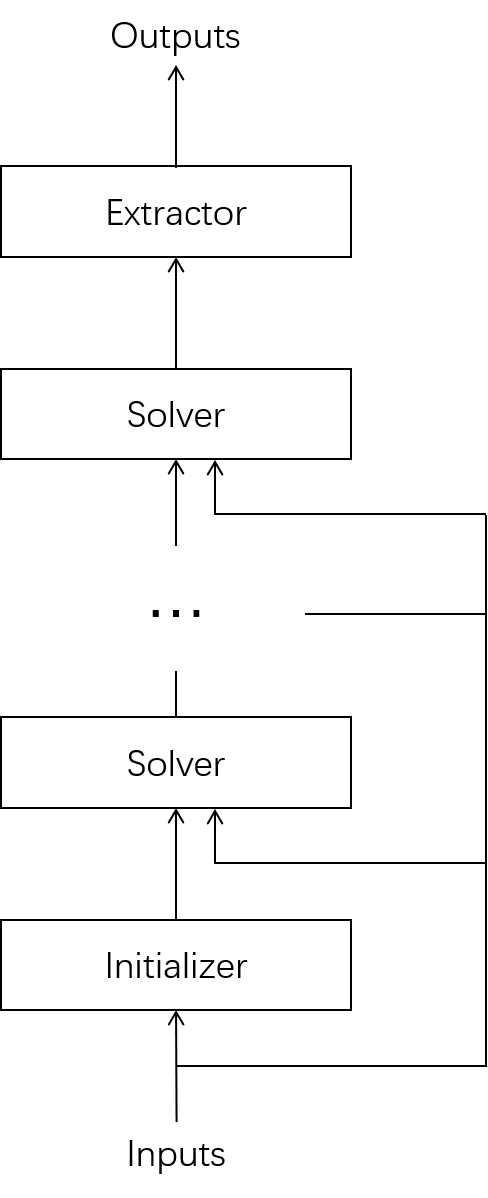
\includegraphics[width=.4\linewidth]{../image/model.png}
			\caption{GenCNN Architecture}
			\label{fig:fig1}
		\end{minipage}%
		\begin{minipage}{.5\textwidth}
			\centering
			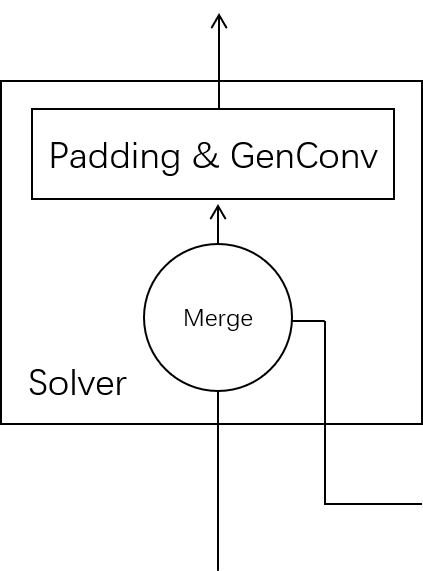
\includegraphics[width=.6\linewidth]{../image/solver.png}
			\caption{Solver Architecture}
			\label{fig:fig2}
		\end{minipage}
	\end{figure}


\end{frame}

\begin{frame}{Build GenCNN}

	ReLU and Linear layer can do a lot of things!

	Notice that 
    
    $$\min(a, b) = a - relu(a - b)$$

    $$1_{a<b} = min(relu(b-a)*10000,1)$$

	We can build GenKernel with a MLP with relu activation function.

    We can use similiar tricks to build Extractor.

\end{frame}

\begin{frame}{More Generalized GenCNN}

	A more generalized GenCNN has a preparer part to do features pre-extraction.

	We need a good global inputs.

	Also, $d[i,j]$ can be a vector instead of a number.

	\begin{figure}[H] %H为当前位置,!htb为忽略美学标准,htbp为浮动图形
		\centering %图片居中
		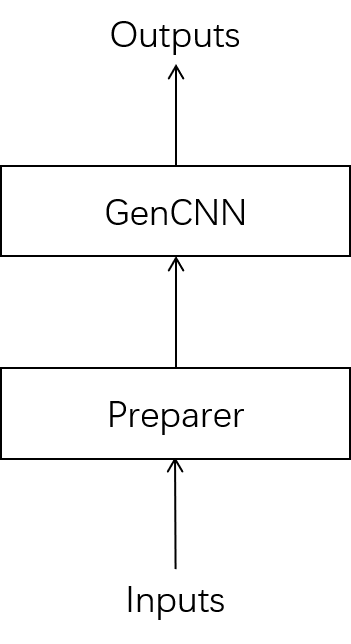
\includegraphics[width=0.2\textwidth]{../image/gen.png} %插入图片,[]中设置图片大小,{}中是图片文件名
		\caption{Generalized GenCNN Architecture} %最终文档中希望显示的图片标题
		\label{Fig.GenCNN} %用于文内引用的标签
	\end{figure}

\end{frame}

\section{Discussion}

\begin{frame}{GenCNN vs CNN}


    \begin{block}{Global Inputs}

        GenCNN has global inputs, like a deep ResNet, but works very differently.

        CNN only uses the previous layer to predict the next layer.

	\end{block}

    \begin{block}{GenKernel}

        GenCNN use GenKernel $x_{new} = f(X)$.
    
        CNN use Kernel $x_{new} = \sigma(\Sigma w_ix_i + b)$.

	\end{block}

	\textbf{Claim: GenCNN is similiar to GCN!}

\end{frame}

\begin{frame}{Advantages of Global Inputs }

	\textbf{Global Inputs}:

	It will not be so smooth because we changed the fixed point.

	Can be used to improve GCN and CNN!

\end{frame}

\begin{frame}{Advantages of GenKernel}

	\textbf{GenKernel}:

	\begin {itemize}

	\item GenKernel can build all cellular automata!

	\item More Expressive!

	\item Wider inductive bias!

	\item More than image ...

	\end {itemize}


\end{frame}


\begin{frame}{Areas for Improvement}


    \begin{block}{Depth}

        GenCNN is too Deep!

        Reason: No dynamic loop structure in the network.

	\end{block}

    \begin{block}{Speed}

        GenKernel is too slow if we use MLP.

        Can we have a GenKernel different from Kernel but have the same speed and good result?

    \end{block}

\end{frame}


\begin{frame}{Areas for Improvement}

    \begin{block}{Initializer}

        Initializer is not expressed by neural network in GenCNN for cycle dataset, but by hard logic.

    \end{block}

    \begin{block}{Dataset}

        We need more harder deterministic dataset.

    \end{block}

\end{frame}


\begin{frame}

	\thispagestyle{empty}

	\begin{center}

		\Huge{Questions?}

	\end{center}

\end{frame}

%%%%%%%%%%%%%%%%%%%%%%%%%%%%%%%%%%%%%%%%%%%%%%%%%%%%%%%%%%%%%%%%

\end{document}